\chapter{Revisión sistemática basada en evidencia}\label{chap_RSBE}

En este proyecto se realizó una revisión sistemática basada en evidencia científica relacionada al uso de sensores IMU para analizar la marcha de las personas al caminar. Conforme a los requerimientos del proyecto, el objetivo de la revisión sistemática se centró en identificar todo el material relevante que permita estudiar la marcha de las personas con el uso de sensores, reducir o eliminar incertidumbres en la investigación, y sobre todo no reinventar la rueda. El conocimiento recopilado fue fundamental para la implementación de la solución PARKIBIP, para mejorar la marcha de los pacientes con la enfermedad de Parkinson.

\section{Planeamiento y diseño de Protocolo de Revisión}

Es esencial para alcanzar resultados satisfactorios establecer un plan, llamado protocolo de revisión, con todas las actividades a realizar y criterios a utilizar previo a la ejecución de la SLR. Desarrollar dicho plan, permite guiar y registrar las estrategias y toma de decisiones de diseño del estudio (es decir, es el documento de referencia).

A su vez, la actividad de planeación incluye definir las preguntas de investigación y desarrollar la estrategia de búsqueda, los criterios de inclusión/exclusión, el formulario de extracción de datos, ente otros.

De esta manera, a través de un proceso iterativo y mediante la participación activa de todos los miembros del equipo en el desarrollo, se estableció un protocolo de revisión en una hoja de cálculos tabulada. Resultó esencial para su construcción la realización de diversas pruebas piloto con el mismo que permitan encontrar inconsistencias en los procedimientos de recolección y agregación de los datos. 

Para establecer el objetivo de la revisión sistemática, se plantean cuatro preguntas de investigación que guían la revisión:

\begin{itemize}
    \item ¿Qué tipo de sensores IMU se utilizan para medir la marcha de las personas?
    \item ¿Cuántos sensores son necesarios para medir las características de la marcha?
    \item ¿Qué datos sobre la marcha se pueden obtener con los distintos sensores?
    \item ¿Qué técnicas o algoritmos se utilizan para analizar y procesar los datos?
\end{itemize}

La tabla Tab. \ref{tab_protocolcomponents_PARKIBIP} resume los componentes del protocolo, especifica los métodos que se utilizarán para llevar a cabo la SLR; su definición de antemano ayuda a reducir la probabilidad de sesgo en la investigación. 

\begin{longtable}[p{15cm}]{|p{5cm}|p{10cm}|}
\hline
\multicolumn{2}{| c |} {\textbf{1. Contexto}}  \\ \hline
\textbf{1.1. Objetivo} & Investigar el uso de sensores IMU para analizar la marcha de las personas al caminar\\\hline
\textbf{1.2. Necesidad} & Se quiere mejorar la marcha de las personas con enfermedad de Parkinson, por lo que se quiere relevar la forma de estudiar la marcha de las personas con el uso de sensores\\ \hline
\textbf{1.3. Preguntas de investigación} & \\ \hline
RQ1 & Qué tipo de sensores IMU se utilizan para medir la marcha de las personas?\\ \hline
RQ1.1 & Cuántos sensores son necesarios para medir la marcha? \\ \hline
RQ1.2 & Qué datos sobre la marcha se pueden obtener con los distintos sensores?\\ \hline
RQ1.3 & Qué técnicas o algoritmos se utilizan para analizar y procesar los datos?\\ \hline
%Start Search strategy 
 \multicolumn{2}{| c |}{\textbf{2. Proceso de Búsqueda}}\\ \hline
\textbf{2.1. Estrategia} & Búsqueda automática en título, abstract y keyworkds filtrado por diciplina\\ \hline
\textbf{2.2. Snowballing} & No\\ \hline
\textbf{2.3. Términos} & \\ \hline
Gait analysis & Gait analysis, step analysis, step detection, gait detection\\ \hline
Inertial measurement unit & IMU, Inertial measurement unit\\ \hline
Foot-ground contact & Foot-ground contact, foot ground detection, FGCD\\ \hline
\textbf{2.4. Cadena de Búsqueda} & TITLE-ABS-KEY ( ( ``gait analysis''  OR  ``step analysis''  OR  ``step detection''  OR  ``gait detection'')  AND  ( ``imu''  OR  ``inertial measurement unit'' )  OR  ( ``foot ground contact''  OR  ``foot-ground contact''  OR  ``foot ground detection''  OR  ``FGCD'' ) )  AND  PUBYEAR  $>$  2015  AND  ( LIMIT-TO ( SUBJAREA ,  ``ENGI'' )  OR  LIMIT-TO ( SUBJAREA ,  ``COMP'' )  OR  LIMIT-TO ( SUBJAREA ,  ``BIOC'' )  OR  LIMIT-TO ( SUBJAREA ,  ``MEDI'' ) )\\ \hline
\textbf{2.5. Motores y Cadenas de Búsqueda} & Portal Timbó, Scopus, ScienceDirect\\ \hline
\textbf{2.6. Fuentes a considerar} & N/A\\ \hline
\textbf{2.7. Período a tener en cuenta} & Debido a la evolución de las tecnologías, sensores y aplicaciones se consideran solamente los artículos con año de publicación 2016-2019\\ \hline
\textbf{2.8. Procedimientos auxiliares} & N/A\\ \hline
\textbf{2.9. Evaluación del Proceso de Búsqueda} & Muy bueno. Se logro obtener un numero adecuado de artículos seleccionados con posible buen aporte.\\ \hline
%Start selection process
 \multicolumn{2}{| c |}{\textbf{3. Proceso de Selección de Estudios Primarios}}\\ \hline
\textbf{3.1. Criterios de Inclusión} & Que sea completo. Que se tenga acceso al artículo. Estudios en Ingles, Español y Portugués. Año de publicación $>$ a 2015.\\ \hline
\textbf{3.2. Criterios de Exclusión} & Que no sean papers científicos o con el formato incorrecto. Que no traten la marcha de personas. Que usen sensores difíciles de acceder. Descartar estudios duplicados. Que usen sensores que no sean IMU. Que se enfoquen en la posición en la que se encuentra el sujeto y no en los parámetros de la marcha\\ \hline
\textbf{3.3. Roles de los revisores} & Ambos revisores realizarán las mismas tareas de forma equitativa. Selección, extracción y síntesis.\\ \hline
\textbf{3.4. Cómo se evaluará el acuerdo entre revisores} & Coeficiente de acuerdo Kappa\\ \hline
\textbf{3.5. Cómo se resolverán diferencias} & Discusión abierta en busca de un acuerdo. En caso de no llegar al acuerdo sera excluido.\\ \hline
\multicolumn{2}{| c |}{\textbf{4. Proceso de Evaluación de la Calidad de los Estudios}}\\ \hline
\textbf{4.1. Se evaluará la calidad de los estudios (justificar)} & Si. \\ \hline
\textbf{4.2. Lista de Verificación propuesta (del ingles, Checklist)} & En esta etapa se utilizará la técnica de evaluación Scoring, la cual consiste en plantear una checklist y asignarle a cada ítem el valor 0 ó 1. Luego, se suma el puntaje obtenido para la checklist y se discute la exclusión del articulo.\\ \hline
\textbf{4.3. Cómo se evaluará el acuerdo entre revisores} & N/A\\ \hline
\textbf{4.4. Cómo se resolverán diferencias} & Discusión abierta en busca de un acuerdo. En caso de no llegar al acuerdo el articulo será excluido.\\ \hline
\multicolumn{2}{| c |}{\textbf{5. Proceso de Extracción de Datos}}\\ \hline
\textbf{5.1. Formulario de extracción} & Se establece un formulario en formato tabular que indica los campos de interés que direccionan las preguntas de investigación.\\ \hline
\textbf{5.2. Estrategia de extracción} & División equitativa de artículos. Revisiones de a pares en base a 1 articulo aleatorio.\\ \hline
\textbf{5.3. Consideraciones adicionales (datos calculados, subjetivos, etc.)} & El proceso sera proactivo y abierto a la inclusión de características que se consideren relevantes. Además, se pretende obtener un listado de tipos y/o marcas de los IMU, para luego realizar una comparación.\\ \hline
\multicolumn{2}{| c |}{\textbf{6. Proceso de Síntesis de Datos}}\\ \hline
\textbf{6.1. Tipo de Síntesis} & Se realiza una síntesis temática.\\ \hline
\textbf{6.2. Forma de validación de la síntesis} & N/A\\ \hline
\caption{\label{tab_protocolcomponents_PARKIBIP} Componentes del protocolo de revisión de PARKIBIP.}
\end{longtable}

\noindent Tal como se puede apreciar en la tabla, la misma se encuentra segmentada en distintas etapas, siendo consistente con las principales etapas de una SLR estándar.

\section{Estrategia de búsqueda}

Se planeó una estrategia de búsqueda automatizada, en función de la definición de una cadena de búsqueda que incluya la combinación de las palabras claves del problema de estudio, así como también sus alias (p. ej. Gait Analysis, IMU, etc.). Para ello, se seleccionaron los servicios de indexamiento y librerías digitales a través de portal Timbó (e.g, Scopus, IEEE, Springer Link), como motores de búsqueda principales.

Los términos de búsqueda utilizados se construyeron siguiendo los siguientes pasos:
\begin{enumerate}
    \item Definir los términos principales
    \item Identificar ortografías alternativas, sinónimos o términos relacionados para términos principales
    \item Verificar las palabras claves en los documentos relevantes previamente identificados
    \item Se usa el OR booleano para incorporar ortografías alternativas, sinónimos o términos relacionados
    \item Se usa el booleano AND para vincular los términos principales
\end{enumerate}


Es de gran importancia resaltar la codificación de la Cadena de búsqueda, la cual es imprescindible para ejecutar una búsqueda automatizada, y que de su buena formación dependerán los resultados futuros (i.e. una malformación de la cadena de búsqueda podrá alcanzar estudios irrelevantes, demasiados o una poca cantidad de los mismos). 
\newline
\noindent\fbox{
     \parbox{\textwidth}{
    \textit{
    TITLE-ABS-KEY ( ( ``gait analysis''  OR  ``step analysis''  OR  ``step detection''  OR  ``gait detection'')  AND  ( ``imu''  OR  ``inertial measurement unit'' )  OR  ( ``foot ground contact''  OR  ``foot-ground contact''  OR  ``foot ground detection''  OR  ``FGCD'' ) )  AND  PUBYEAR  $>$  2015  AND  ( LIMIT-TO ( SUBJAREA ,  ``ENGI'' )  OR  LIMIT-TO ( SUBJAREA ,  ``COMP'' )  OR  LIMIT-TO ( SUBJAREA ,  ``BIOC'' )  OR  LIMIT-TO ( SUBJAREA ,  ``MEDI'' ) )}
    }
}

\section{Criterios de inclusión/exclusión}

Se formularon criterios de selección de artículos a incluir en la revisión, con el fin de identificar aquellos estudios que proporcionen información relevante a las preguntas de investigación y eliminar estudios arbitrarios. Dichos criterios fueron expresados como dos conjuntos, criterios de inclusión y de exclusión, ilustrados en la Tabla \ref{TAB: criterios}.


\begin{table}[H] 
\caption{Criterios de selección de estudios primarios}
\centering
\hspace*{-1cm}%
\begin{tabular}{|p{7cm}|p{8cm}|}
\hline
\textbf{Criterios de inclusión} & \textbf{Criterios de exclusión}\\ \hline
Estudios completos & Estudios arbitrarios -no científicos- o con el formato incorrecto\\ \hline
Con acceso al artículo completo & No traten la marcha de personas\\ \hline
Escritos en los idiomas inglés, español y portugués  & Usen sensores que no sean IMU o difíciles de acceder\\ \hline
Publicados a partir del año 2015 & Se descartan estudios duplicados\\ \hline
    & Se enfoquen en la posición en la que se encuentra el sujeto y no en los parámetros de la marcha \\\hline
\end{tabular}
\hspace*{-1cm}
\label{TAB: criterios}
\end{table}

Asimismo, a través de la cadena de búsqueda se limitan aquellos estudios pertenecientes a las áreas de conocimiento Ingeniería, y/o Computación, y/o Medicina, y/o Bio-ciencias.

\section{Selección}

El propósito de esta etapa es recopilar estudios primarios que proporcionan evidencia directa acerca de las preguntas de investigación.
En primera instancia, los resultados primarios obtenidos fueron evaluados utilizando el título y el resumen del estudio para excluir aquellos que son claramente irrelevantes. Los documentos marginales o para los cuales la inclusión/exclusión es incierta, fueron mantenidos en el conjunto selección y la decisión final fue tomada durante la extracción de datos. Posteriormente, se aplicaron los criterios de selección establecidos iniciando la Selección de estudios relevantes para el proyecto. 

Para llevar a cabo este proceso y facilitar la manipulación de los estudios primarios (i.e. búsqueda y filtrado de datos), resultado de la búsqueda automatizada, los mismos fueron tabulados en hojas de cálculos que incluyen la meta-data:

\begin{itemize}
    \item Año (Year)
    \item Título del artículo (Title)
    \item Resumen (Abstract)
    \item Título de la fuente (Source title)
    \item Enlace (Link)
    \item Editorial (Publisher)
    \item Idioma del documento original (Language of Original Document)
    \item Tipo de documento (Document Type)
    \item Tipo de acceso (Access Type)
    \item Fuente del artículo (Source)
    \item Autores (Authors)
    \item Inclusión
    \item Motivo exclusión
    \item Observación del Articulo
\end{itemize}

El proceso de Selección se realizó en varias etapas, partiendo de 493 artículos que fueron arrojados por la búsqueda automatizada. Aplicando los criterios de selección establecidos, se conformo una lista de 165 estudios, que actuó como entrada de datos para la tarea ``lectura rápida''.  De esta manera, leyendo únicamente el título y el resumen de cada artículo se realizó una primera selección, recopilando alrededor de 85 artículos relevantes para PARKIBIP. A partir de este punto, cada estudio preseleccionado fue identificado unívocamente en el Universo con un identificador auto-incremental.

Luego, leyendo nuevamente el título y el resumen del articulo a evaluar, fueron valorados o puntuados en una escala del 1 al 3, siendo los de categoría 1 aquellos que en primera instancia parecieran ser muy útiles y los de categoría mas alta los que si bien aportaban valor no serían tan relevantes. En este sentido, fue difícil establecer la categoría de ciertos artículos en base al titulo y su resumen, por lo que en una tercera etapa se leyeron cerca de 40 artículos para establecer su categoría (principalmente las secciones de objetivos del artículo, metodología y resultados). Ambos miembros del equipo realizaron esta tarea para revisar y justificar los desacuerdos, de esta forma se alinearon criterios. 

En resumen, el resultado de la fase de Selección se puede visualizar en la tabla \ref{tab:selection_results}.

\begin{table}[H] 
\caption{Resultados del proceso de Selección de estudios. primarios}
\centering
\begin{tabular}{| p{6cm} | p{4cm} |}
\hline
\textbf{Categoría o valoración} & \textbf{Resultado}\\ \hline
1 (relevancia máxima) & 30 estudios\\ \hline
2 (relevancia intermedia) & 22 estudios\\ \hline
3 (relevancia mínima) & 33 estudios \\ \hline
\end{tabular}
\label{tab:selection_results}
\end{table}

\section{Evaluación de calidad}

De la misma forma que se establecieron criterios de inclusión y exclusión para el proceso de selección, es importante establecer criterios para evaluar la calidad de los artículos seleccionados. Mediante la evaluación de estos criterios se descartan los estudios que no son válidos o son subjetivos. La evaluación de la calidad es una etapa relevante ya que la excelencia de los estudios primarios puede incidir en la calidad de los resultados obtenidos.

Para ésta tarea se utilizó la técnica de ``scoring'', la cual consiste en puntuar los artículos según determinados criterios preestablecidos. Los criterios están dados por el conjunto de interrogaciones:
\begin{itemize}
    \item ¿El artículo se encuentra basado en investigación?
    \item ¿Es claro el objetivo del artículo?
    \item ¿Hay una descripción adecuada acerca del contexto en el cual se realizó la investigación?
    \item ¿Se diseñó la investigación de manera correcta para cumplir con el objetivo del artículo?
    \item ¿Hubo alguna replicación, por ejemplo múltiples casos de prueba?
    \item ¿Hay una descripción clara de los hallazgos?
    \item ¿Los hallazgos son de valor para la industria o para investigadores?
\end{itemize}

De esta manera, para cada artículo se respondieron dichas preguntas con una valoración de 1 si la respuesta era afirmativa o en caso contrario 0. Luego, el puntaje de calidad del artículo es la suma de todos las valoraciones, por lo que cada artículo obtuvo un puntaje de 0 a 7. Se excluyen aquellos artículos cuya puntación fue menor a los 5 puntos.

\section{Extracción}

El objetivo en esta etapa del proceso de revisión, es la extracción del contenido necesario para direccionar las preguntas de investigación. Para ello, los estudios resultados del proceso de selección, fueron incluidos a la herramienta Mendeley para un mejor seguimiento. Conforme a mantener consistencia a través de los estudios y dentro del equipo de revisores, se utilizó una estrategia de extracción en base a formularios preestablecidos.

De esta manera, se realizó una extracción de datos que incluye detalles generales de la publicación (i.e. titulo, autores, universidad u organización), como también se encuentra basada en temas específicos: (i) Objetivo del estudio; (ii) Características de los sensores utilizados; (iii) Cantidad de sensores necesarios; (iv) Ubicación de los sensores; (v) Fases del paso analizadas; (vi) Algoritmos utilizados; (vii) Características de los sujetos -sanos o con alguna enfermedad-; (viii) Resultados y efectividad. La figura Fig. \ref{fig:extraction} ilustra y ejemplifica el resultado del proceso mencionado.

\begin{figure}[H]
\begin{center}
\makebox[0pt]{\begin{minipage}{1.2\textwidth}%
\hspace*{-1.7cm}%
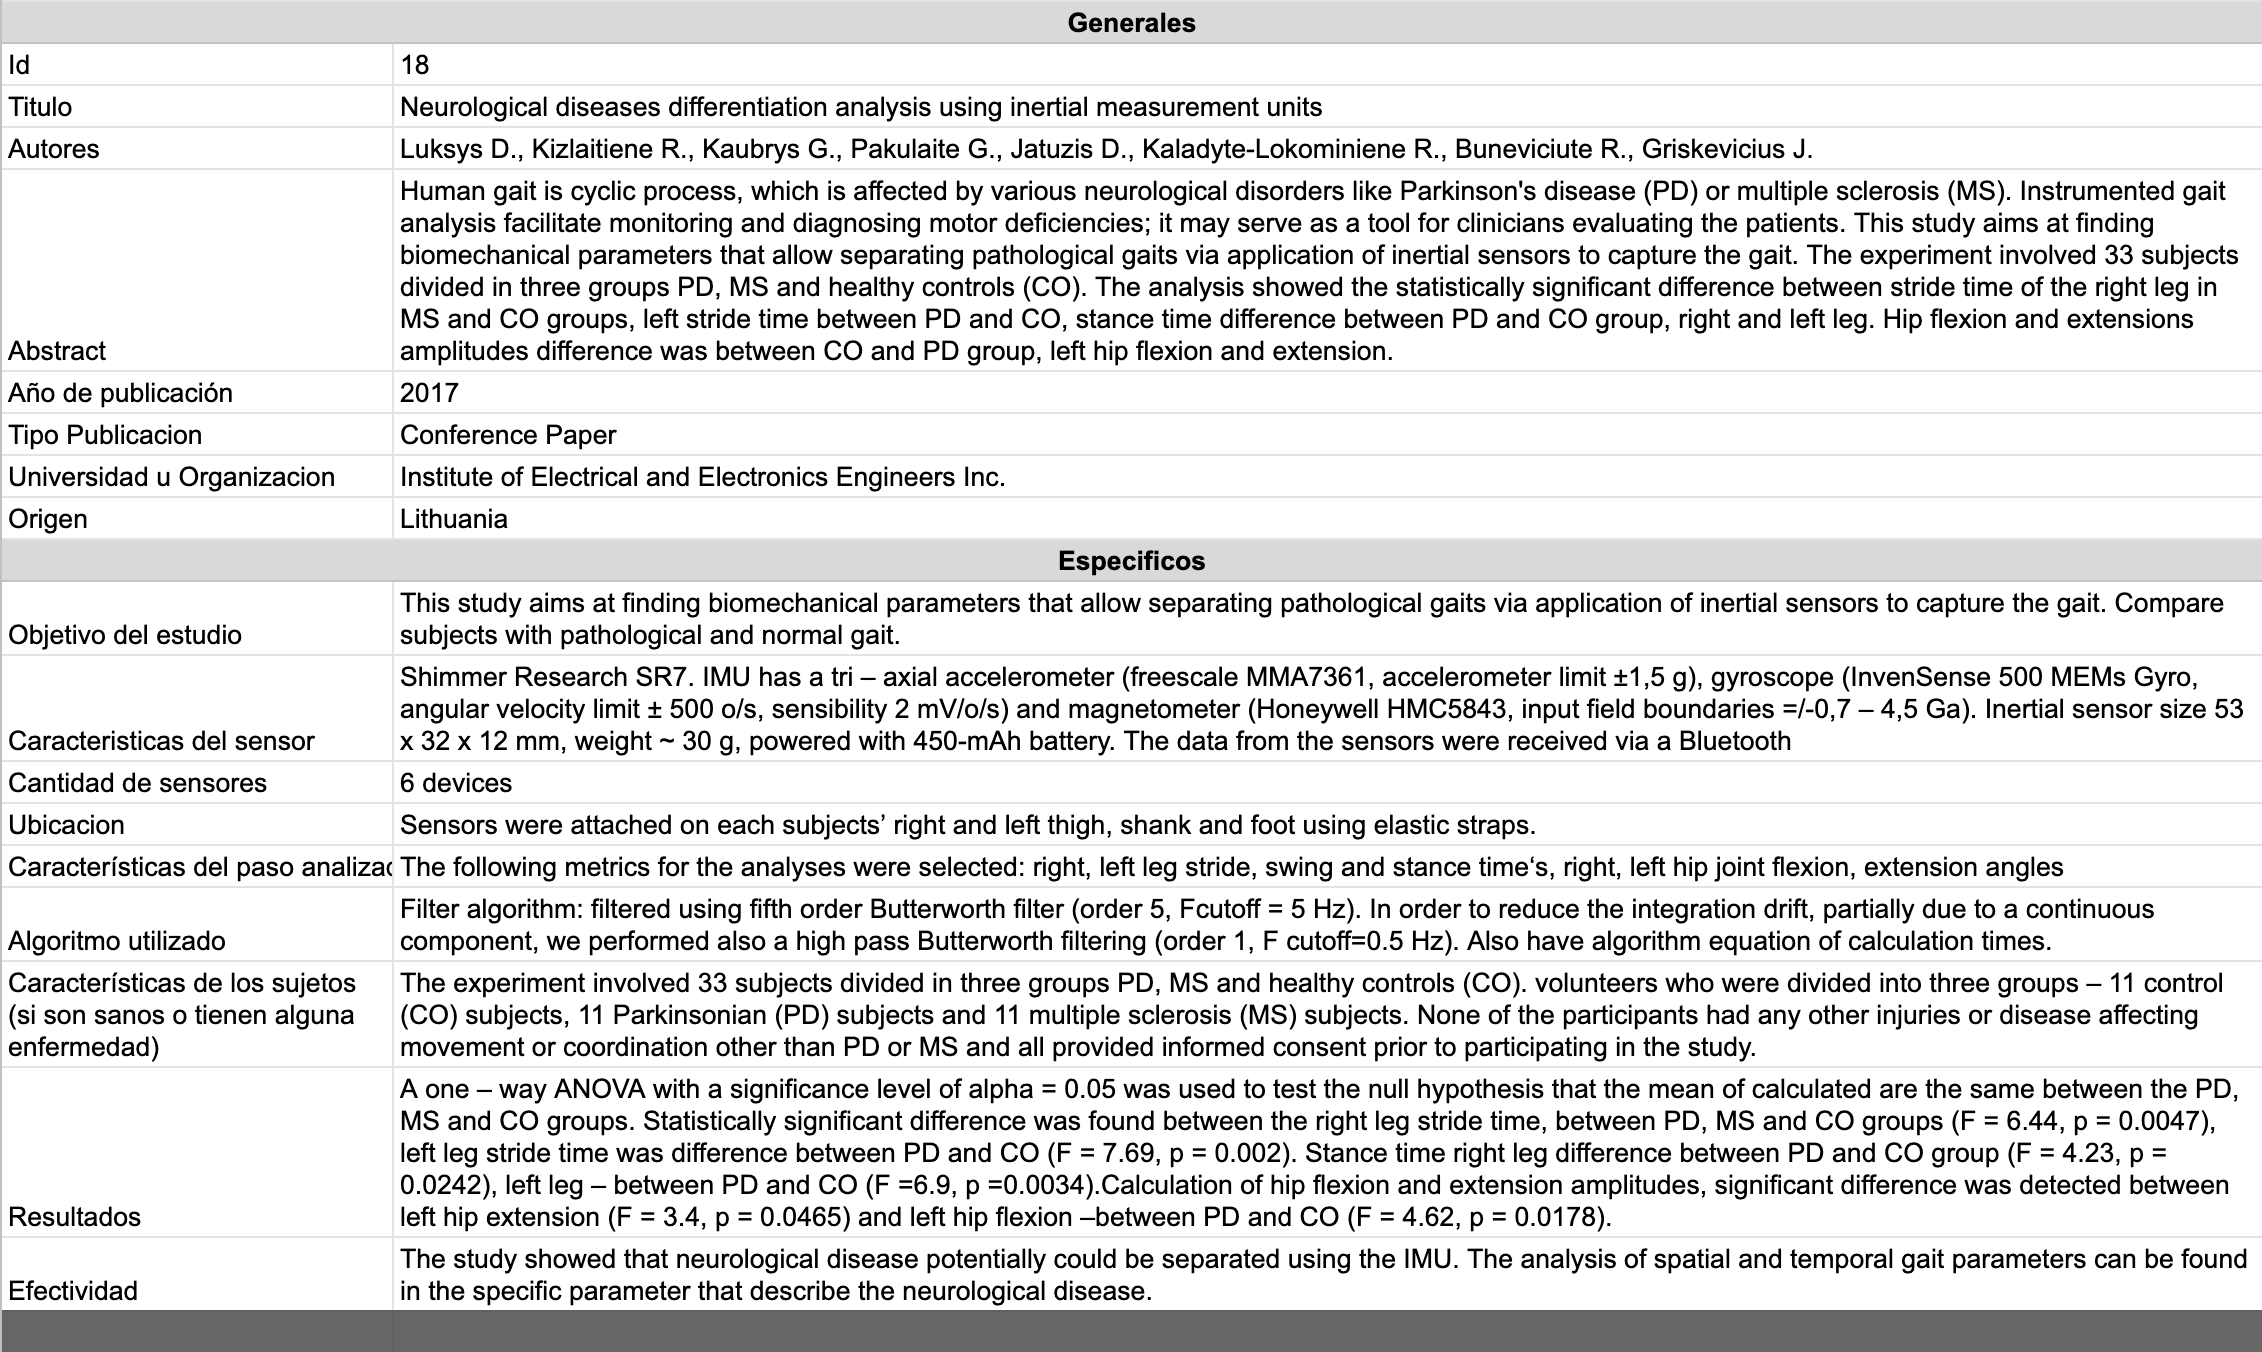
\includegraphics[scale=0.48]{TESIS/imagenes/chap03/extraction-3.png}
\end{minipage}}
\end{center}
\caption{Formulario de extracción empleado en PARKIBIP. }
\label{fig:extraction}
\end{figure} 

\section{Síntesis: Resultados primarios}\label{synthesis}

Teniendo en cuenta el tiempo planificado para la etapa de análisis de la literatura, se priorizó sintetizar el conjunto de investigaciones pertenecientes a la Categoría 1 (30) cuyo aporte tendrá gran relevancia para el proyecto PARKIBIP, tal como indica la tabla Tab.\ref{tab:selection_results}. Con el objetivo de responder las preguntas planificadas se analizó: el año de publicación, el objetivo, las características de los sensores utilizados, la cantidad y ubicación de los sensores, las características del paso analizadas y los algoritmos computacionales empleados para dicho fin, las características de los sujetos -sanos o con alguna patología-.

Más allá del estado del arte respecto al uso de dispositivos IMU para analizar la marcha de las personas al caminar -objetivo central-, resulta útil para los productores y consumidores de la investigación conocer las diversas salidas para la investigación y el crecimiento del campo de estudio. Así, en primera instancia se realizó una clasificación previa de los artículos en base a cuatro criterios:
\begin{enumerate}
    \item Fecha de Publicación
    \item Países involucrados en las investigaciones
    \item Tipo de Publicación
    \item Editorial
\end{enumerate}

%  Fecha de Publicación
La búsqueda realizada se focalizó en los años 2016 al 2019. Esta decisión se debió a que los avances tecnológicos han avanzado considerablemente en los últimos años, por lo tanto, no es relevante para este estudio el análisis de artículos con más de 4 años de antigüedad.
La figura Fig. \ref{fig:synthesis_year} presenta la distribución de estudios primarios por año de publicación. La razón de que exista un único estudio publicado para el año 2019 es trivial -mismo año que la presente LSR-; sin embargo, se observa un buen numero de estudios para los restantes años.

\begin{figure}[H]
\centering
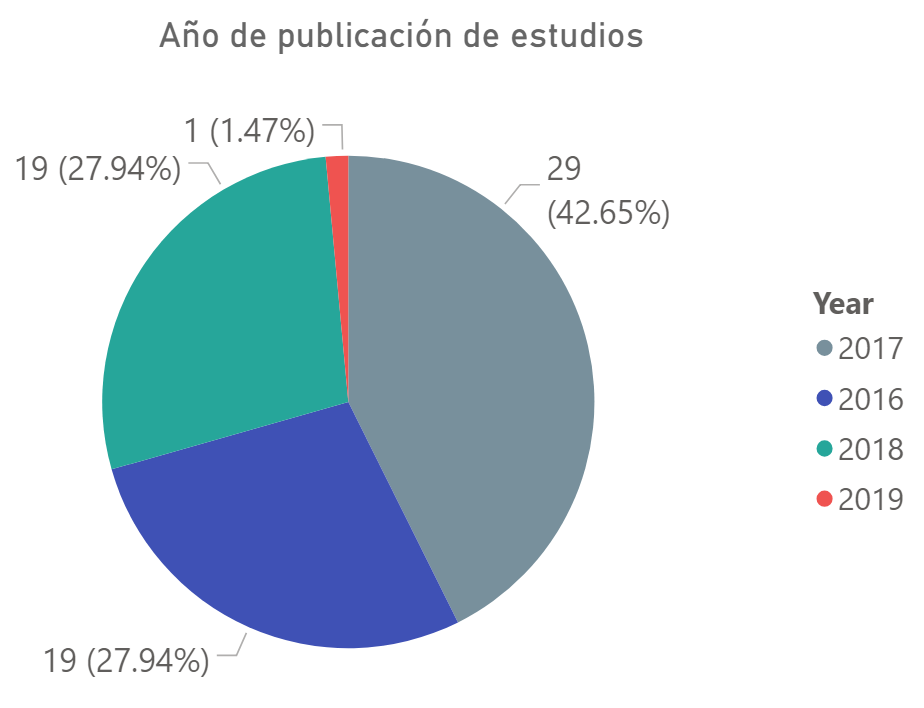
\includegraphics{TESIS/imagenes/chap03/sintesis_anio.PNG}
\caption{Distribución de estudios primarios por año.}
\label{fig:synthesis_year}
\end{figure}

% Países
Resulta importante identificar los países interesados en la materia, ya sea para compartir el conocimiento adquirido y trabajar colaborativamente, o simplemente Benchmarking. En la figura Fig. \ref{fig:synthesis_countries} se presenta la distribución de países involucrados en las investigaciones. Existe una gran prevalencia de investigaciones con origen Italiano (7) indicando un fuerte campo de interés para dicho País. Asimismo, se puede apreciar una buena dispersión de estudios primarios (31) por Países (18) -aprox. 60\% de países distintos-, lo que infiere la importancia compartida del campo de estudio entre países y pocas investigaciones realizadas.    

\begin{figure}[H]
\centering
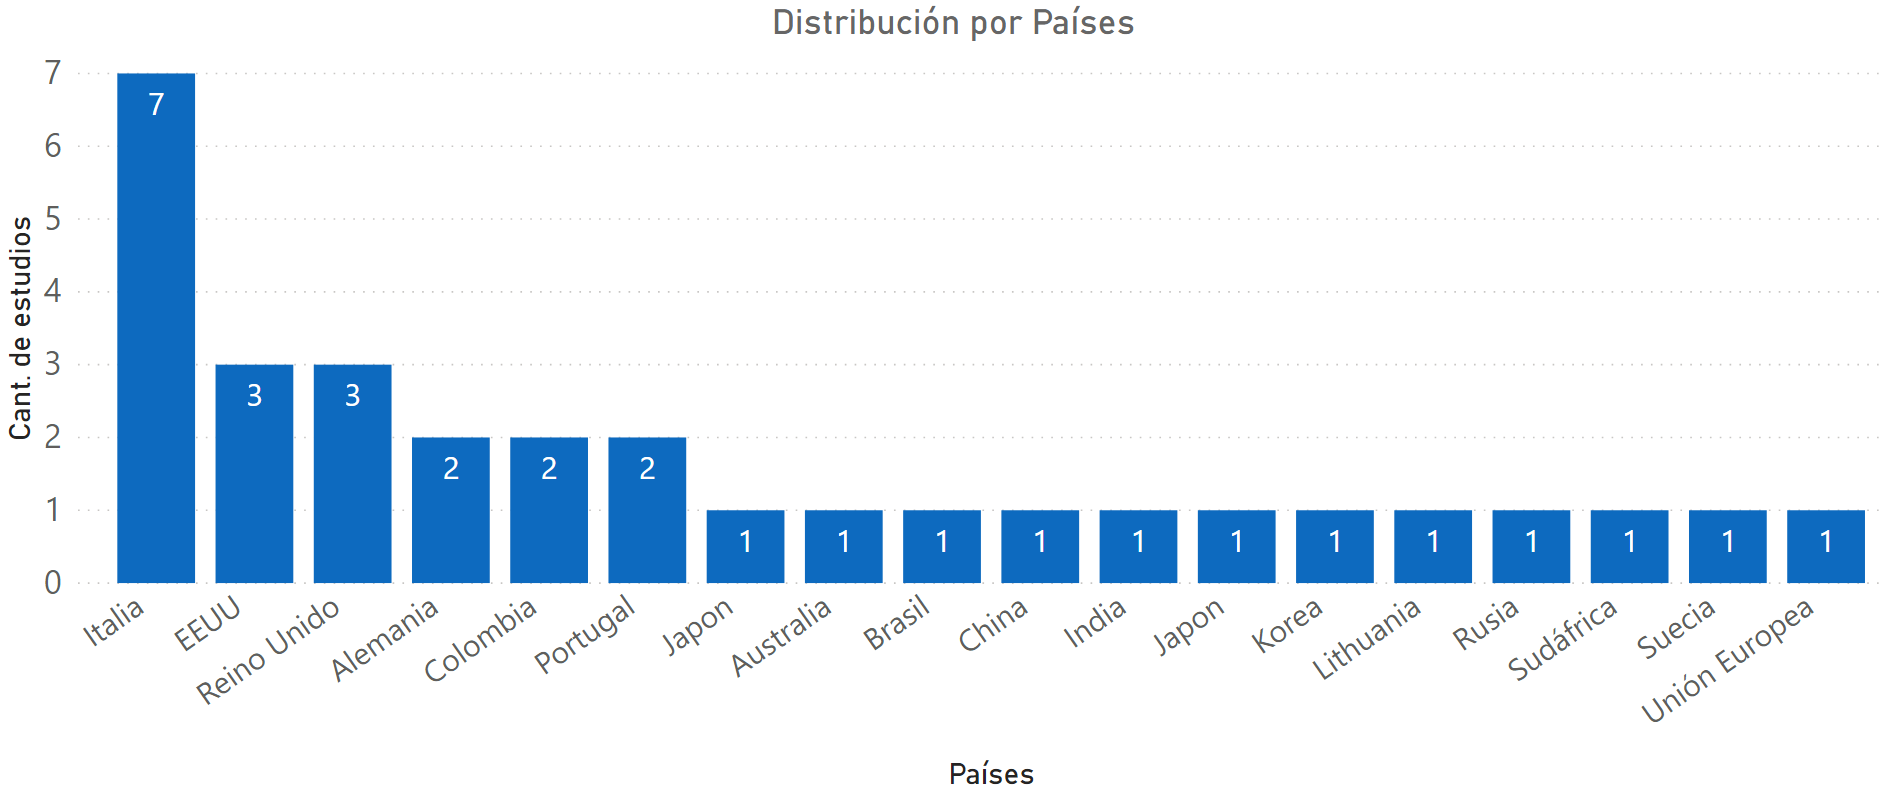
\includegraphics[width=\textwidth]{TESIS/imagenes/chap03/sintesis_country.PNG}
\caption{Gráfico de los países de origen de las investigaciones.}
\label{fig:synthesis_countries}
\end{figure}

% Tipo de Publicación 
Por su parte los artículos analizados fueron publicados tanto en conferencias como en revistas de manera proporcional, con el análisis de una revisión sistemática respecto a las distintas particiones existentes del ciclo de la marcha, y la inclusión del capitulo de un libro. Además, dichas publicaciones fueron fragmentadas por casa editora, siendo la asociación profesional de ingeniería electrónica e ingeniería eléctrica (IEEE) la de mayor presencia con el 50\% de publicaciones aproximadamente. Las figuras Fig. \ref{fig:synthesis_publicationType}\ref{fig:synthesis_publicationEditorial}.

\begin{figure}[H]
\centering
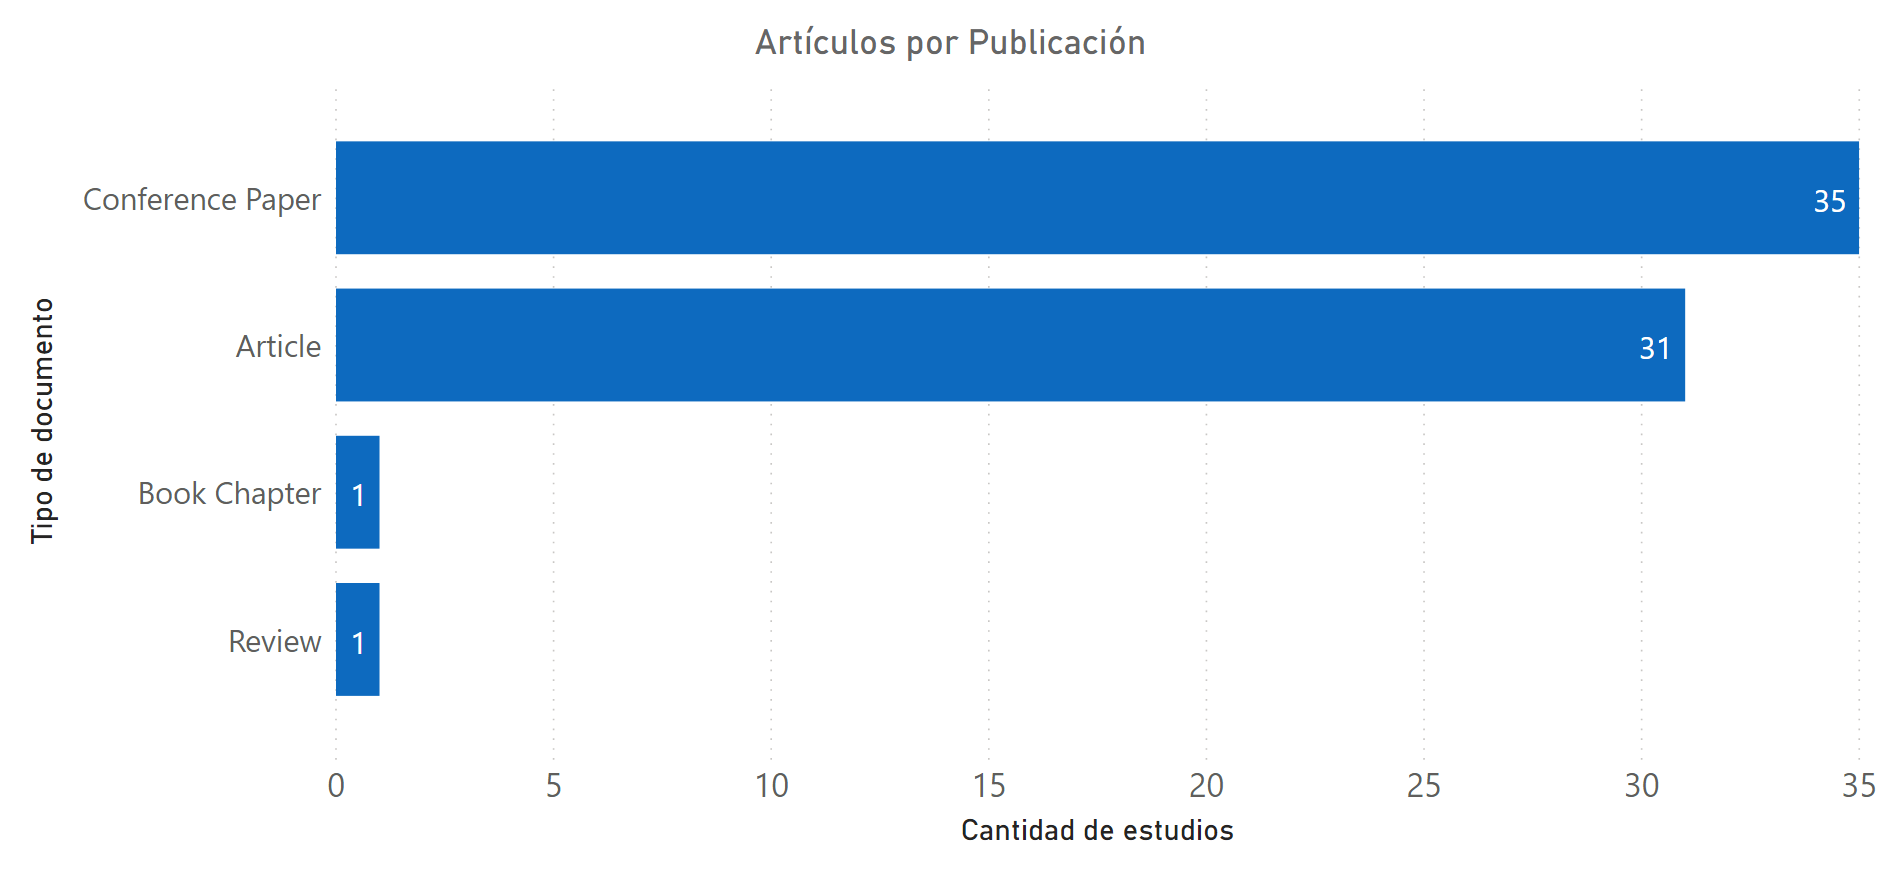
\includegraphics[width=\textwidth]{TESIS/imagenes/chap03/sintesis_documentType.PNG}
 \caption{Artículos sobre análisis de la marcha por tipo de publicación.}
 \label{fig:synthesis_publicationType}
\end{figure}

%Editorial
\begin{figure}[H]
 \centering
 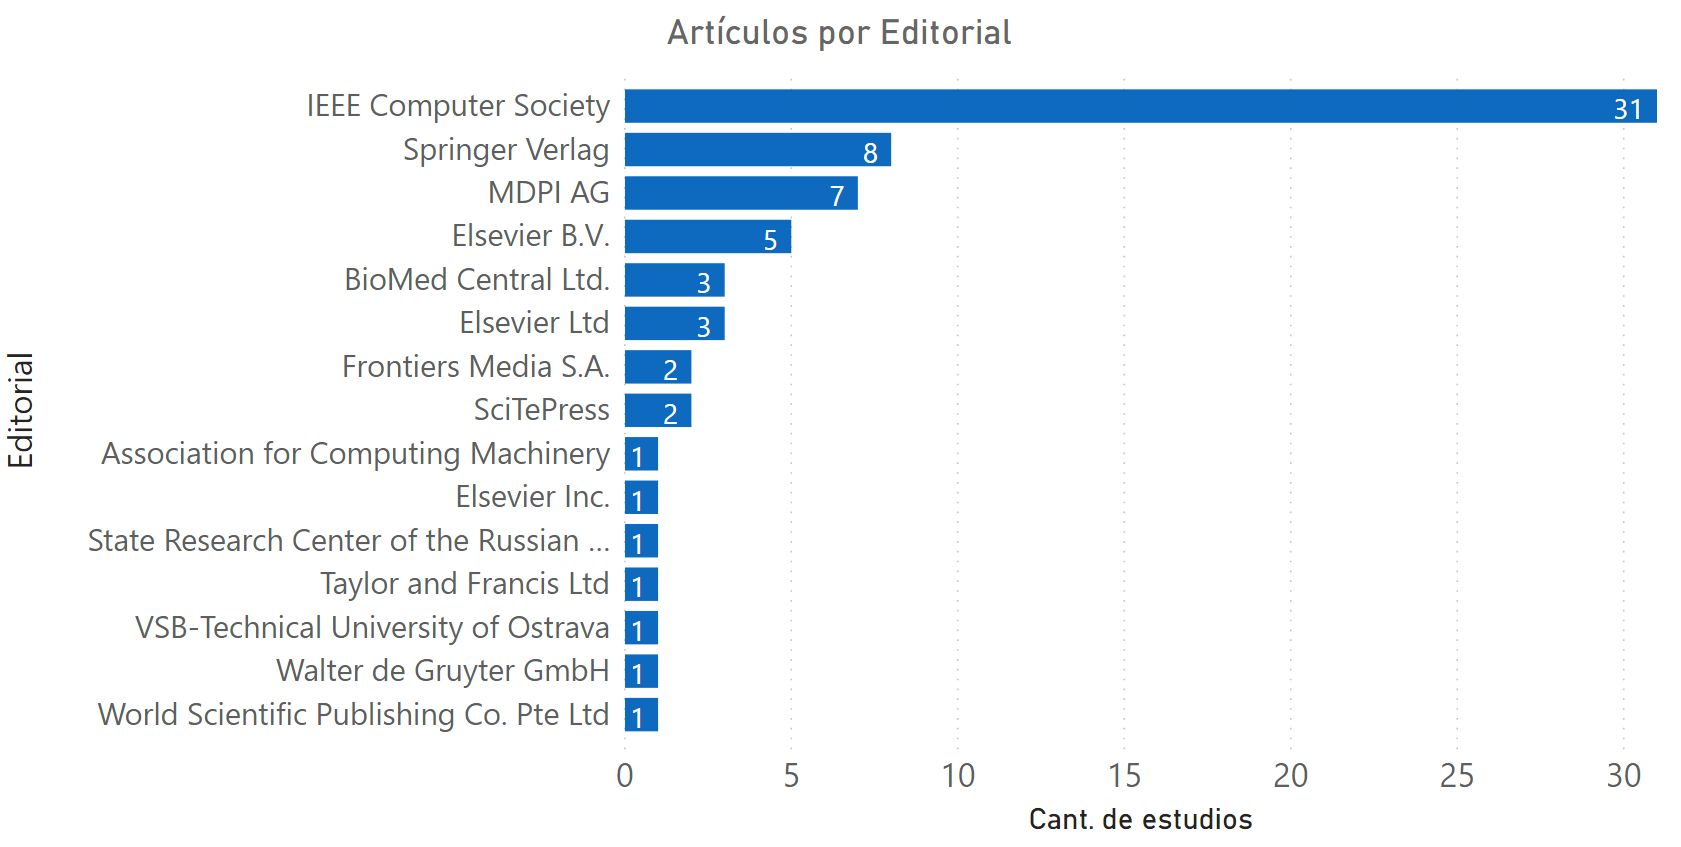
\includegraphics[width=\textwidth]{TESIS/imagenes/chap03/sintesis_editorial.PNG}
 \caption{Artículos sobre análisis de la marcha por editorial.}
 \label{fig:synthesis_publicationEditorial}
\end{figure}

Desde la perspectiva de la revisión sistemática realizada, es importar abordar las preguntas de investigación elaboradas en el objetivo con la finalidad de adquirir conocimiento, contemplar dificultades y riesgos, producir ventajas de la evidencia recolectada.

% 1.Caracteristicas de IMUs
Ya mencionado, los dispositivos IMU pueden contar con diversos sensores de medición; en su forma mas básica cuentan con un acelerómetro. En general, salvo en las investigaciones cuya información no fue especificada, la mayoría de los estudios usaron dispositivos IMU con 9/6 DOF (sus siglas del ingles, refieren a los grados de libertad, variables independientes) de diversas compañías; integrando la combinación de un acelerómetro y giroscopio tridimensionales, en algunos casos también un magnetómetro tridimensional. Es relevante notar que, todos los dispositivos empleados tienen como salida datos en la unidad correspondiente al sensor y sin procesar; de ahí la necesidad de algoritmos específicos al caso de uso.

% 2.Cuántos sensores son necesarios para medir la marcha? 
Según el área de estudio particular dentro de la marcha de las personas, las investigaciones emplearon entre 1 y 7 dispositivos IMU. Aproximadamente el 86.5\% de los estudios requirió dos o mas dispositivos, en donde prevalece con el 50\% el uso de dos dispositivos. La figura Fig. \ref{fig:synthesis_devices} sintetiza el numero de dispositivos que fueron necesarios para realizar cada investigación.

\begin{table}[H] 
\caption{Cantidad de dispositivos empleados para analizar la marcha de personas según los artículos contemplados.}
\centering
\begin{tabular}{| p{4cm} | p{4cm} |}
\hline
\textbf{Dispositivos IMU (en unidades)} & \textbf{Artículos (en unidades)}\\ \hline
1 & 4\\ \hline
2 & 12\\ \hline
3 & 6 \\ \hline
4 & 2 \\ \hline
5 & 1 \\ \hline
6 & 3 \\ \hline
7 & 1 \\ \hline
\textbf{Total} & \textbf{28}\\ \hline
\end{tabular}
 \label{fig:synthesis_devices}
\end{table}

\noindent A priori, se podría concluir que empleando un único dispositivo inercial sería suficiente para analizar la marcha de las personas y elevar los costos y las complejidades con otros adicionales. Sin embargo, éste resultado subjetivo no es correcto; y como fue mencionado, la cantidad de dispositivos necesarios depende de las variables de estudio dentro del ``gait analysis'' -i.e. según partición del ciclo de la marcha, parámetro espacio-temporal particular (aceleración, velocidad, etc.), simetría entre pasos, rotación tobillo, entre otras-. Sumado a la anterior afirmación, se debe contemplar los algoritmos computacionales empleados, la ubicación del dispositivo, la cantidad de variables de la marcha a analizar para dicha ubicación, la efectividad reportada para esa variable de estudio. Por ejemplo, un único dispositivo ubicado en el centro de masa -a la altura de la pelvis- podría detectar si existe movimiento, en cambio, no se podría estudiar el ciclo de la marcha en 2 fases Stance (fase de apoyo) y Swing (fase de vuelo) por pie y por lo tanto limitando los parámetros espacio-temporales de los mismos.

% 3.Que ubicaciones utilizan los dispositivos?
Similar a lo mencionado, la ubicación anatómica del dispositivo en el cuerpo humano tiene gran relevancia y determina/limita el espectro de estudio. La figura Fig. \ref{fig:synthesis_location} con sus respectivas sub-figuras, resume las distintas ubicaciones anatómicas empleadas para posicionar al menos un IMU, así como también sus distintas configuraciones que permiten el ``gait analysis''. Las mismas, exhiben que si bien las posiciones anatómicas son variadas y aproximadamente el 33\% localiza al menos un IMU en la Tibia; según las configuraciones, en su mayoría se localiza únicamente en el pie del sujeto en cuestión.

\begin{figure}
     \centering
     \begin{subfigure}[b]{1\textwidth}
         \centering
         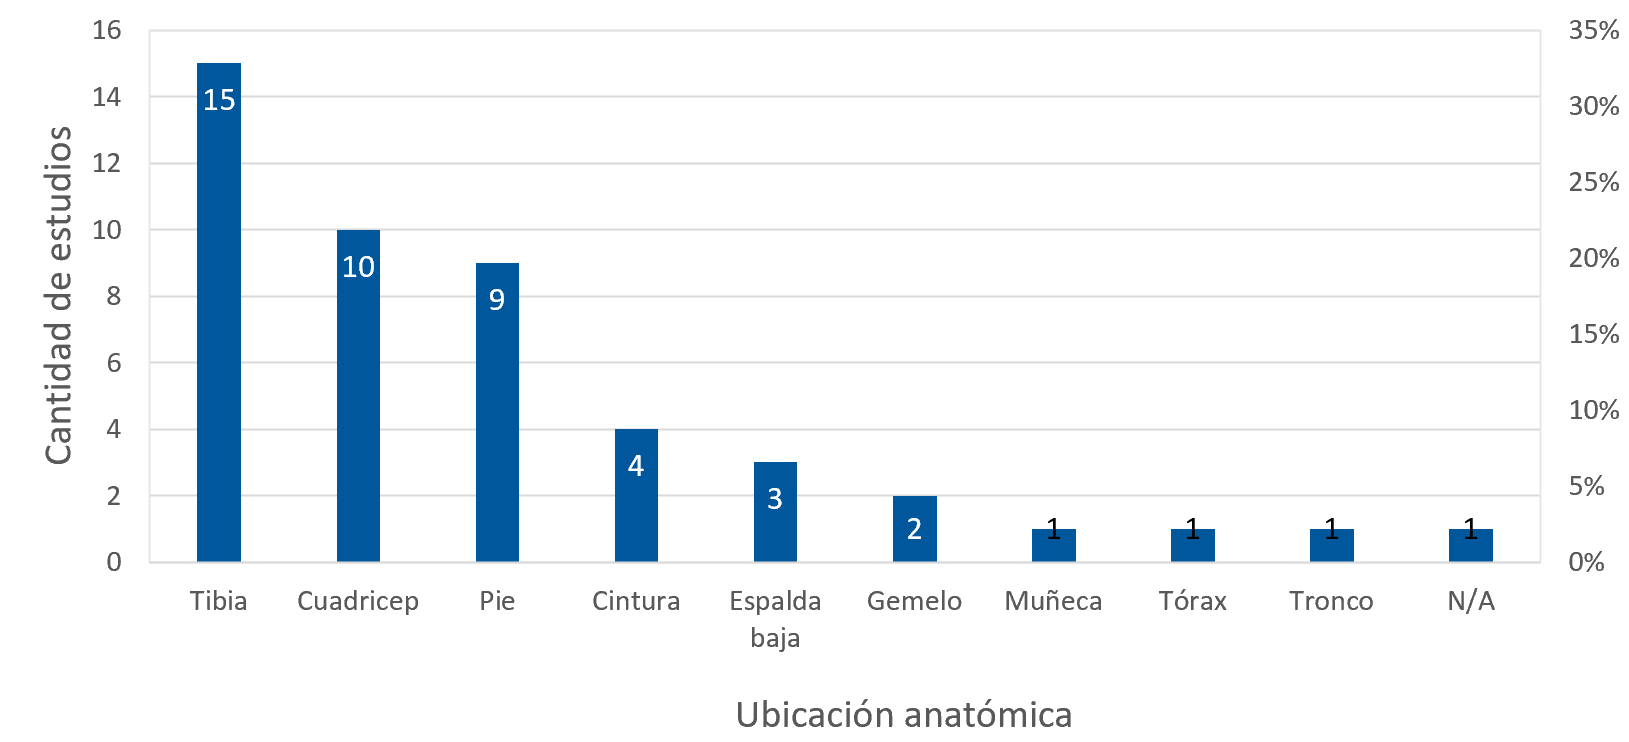
\includegraphics[width=\textwidth]{TESIS/imagenes/chap03/ubicaciones-anatomicas.PNG}
         \caption{Ubicaciones anatómicas empleadas para posicionar al menos un IMU en el análisis de la marcha de personas. Según la evidencia, aproximadamente el 33\% de estudios emplea la Tibia, luego el Cuádricep y el Pie del sujeto con un $\approx$20\%. }
     \end{subfigure}
     \begin{subfigure}[b]{1\textwidth}
        \centering
        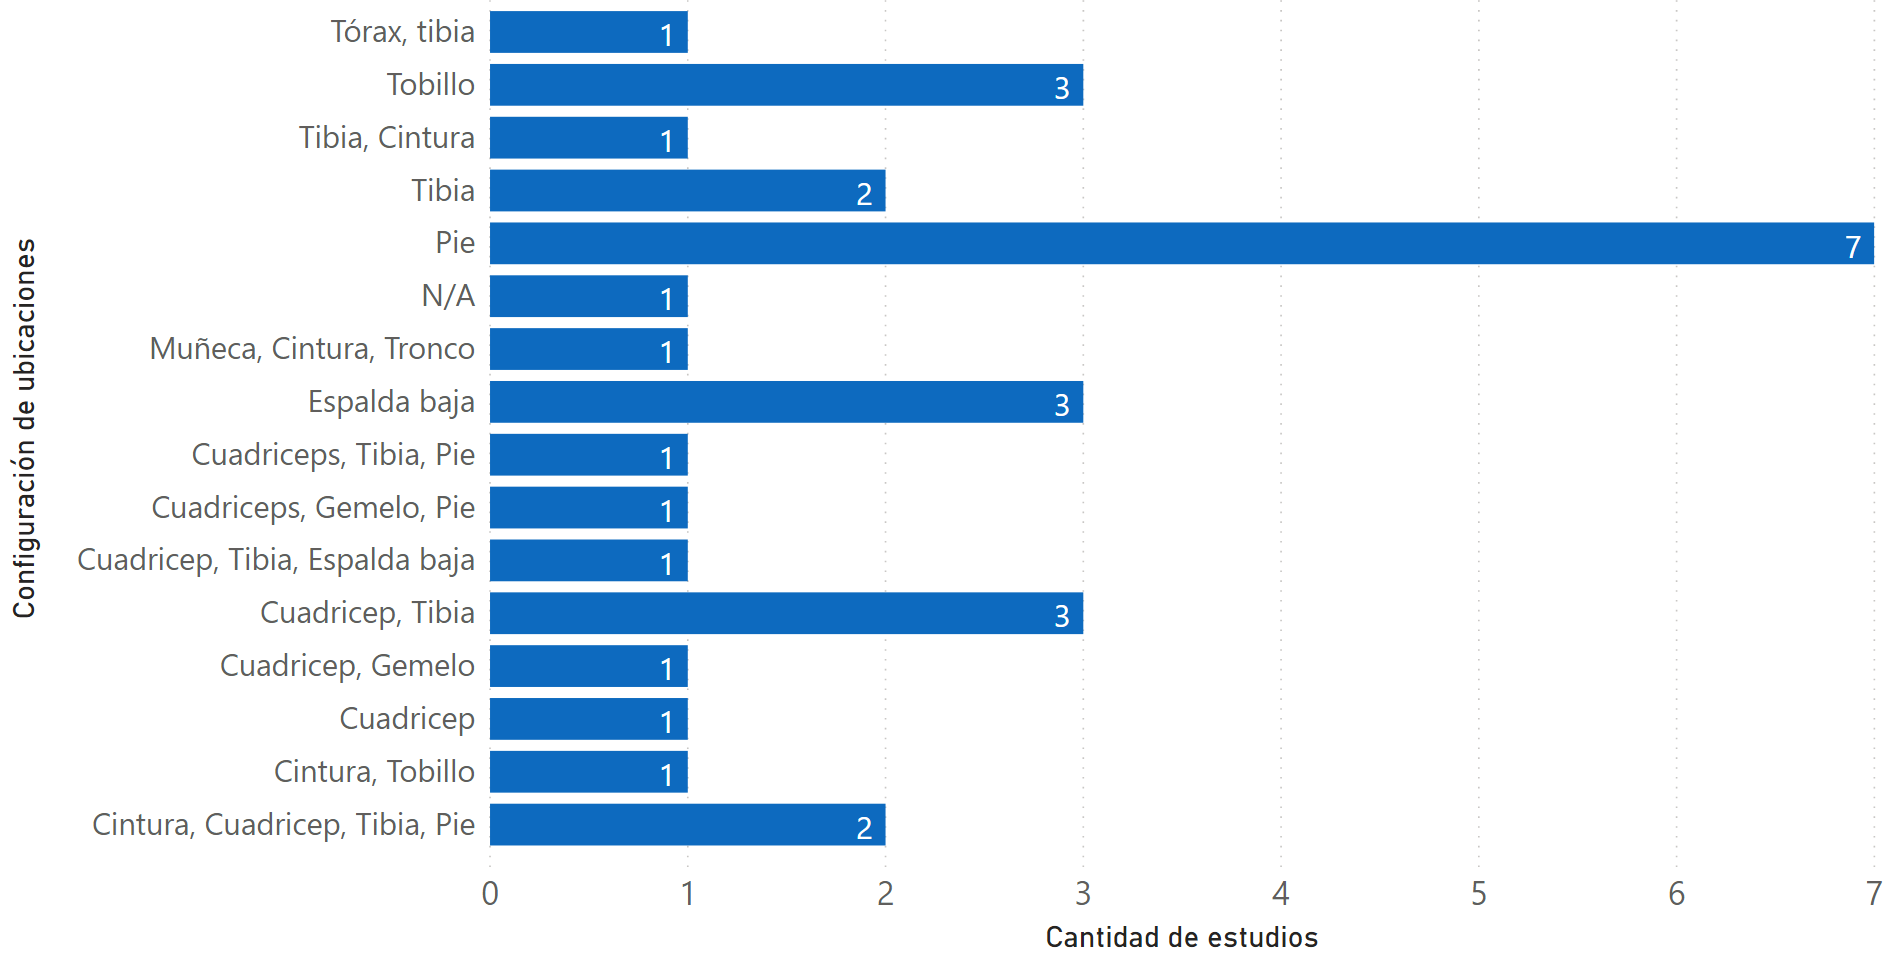
\includegraphics[width=\textwidth]{TESIS/imagenes/chap03/sintesis_location.PNG}
        \caption{Configuraciones de ubicaciones anatómicas para posicionar los IMU que permiten analizar la marcha de un sujeto.}
     \end{subfigure}
     \caption{Ubicaciones de dispositivos IMU en el cuerpo de los sujetos para el análisis de la marcha, según los distintos estudios de la revisión sistemática.}
     \label{fig:synthesis_location}
 \end{figure}


Combinando los resultados anteriores -cantidad y ubicación en el cuerpo- sobre los dispositivos empleados, se puede afirmar que la mayoría de estudios empleó dos dispositivos IMU localizados en el pie del sujeto particular. Además, dicha ubicación permite abordar los problemas esenciales:
\begin{itemize}
    \item Identificar el ciclo de la marcha por extremidad
    \item Estudiar diversos parámetros espacio-temporales por extremidad o de forma general
\end{itemize} 

% 4.Qué datos sobre la marcha se pueden obtener con los distintos sensores?

Por otro lado, resulta crucial para la investigación entender \textbf{de qué forma se procesan los datos}, \textbf{qué eventos se detectan} para distinguir las distintas etapas de la marcha y \textbf{qué tipo de parámetros se pueden obtener} con cada tipo de análisis. La tabla Tab. \ref{tab_synthesis_algorithm} enumera 
los datos mencionados para cada uno de los 30 artículos analizados.

{\fontsize{9}{11}\selectfont
\setlength\LTleft{-2.5cm}
\begin{longtable}{|p{1cm}|p{4cm}|p{2.5cm}|p{3.5cm}|p{6cm}|}
\hline
\label{tab_synthesis_algorithm}
\textbf{ID} & \textbf{Nombre del artículo} & \textbf{Eventos detectados} & \textbf{Algoritmo utilizado} & \textbf{Parámetros obtenidos} \\ \hline
\endhead
1 & Gait evaluation using inertial measurement units in subjects with Parkinson's disease & Heel Strike, Toe Off & Double Integration. High pass filter. Butterworth filter. & Cadence (steps/min). Mean velocity (m/s). Stride length (m). Stride duration (s). Step duration (\%). Stance phase duration (\%). Swing phase duration (\%). Double support phase duration (\%). \\ \hline
2 & Towards a portable human gait analysis \& monitoring system & Heel Strike, Toe Off & Double Differential and Integration, ZUPT & Steps. Kinematic angles in Sagittal, Transverse and Frontal planes. \\\hline
3 & Trainer in a pocket - Proof-of-concept of mobile, real-time, foot kinematics feedback for gait pattern normalization in individuals after stroke, incomplete spinal cord injury and elderly patients & Heel Strike, Toe Off & Kalman Filter - ZUPT & Stride length. Foot to ground angle. Stance time. Swing time \\ \hline
4 & Validity of shoe-type inertial measurement units for Parkinson's disease patients during treadmill walking & Heel Strike, Toe Off
 & Double Integration. Butterworth filter. & Cadence. Step length. Step time \\ \hline
5 & Estimation of spatio-temporal parameters of gait from magneto-inertial measurement units: Multicenter validation among Parkinson, mildly cognitively impaired and healthy older adults & Heel Strike, Toe Off & Custom method* & Stride duration. Step duration. Cadence \\ \hline
6 & Optimal Foot Location for Placing Wearable IMU Sensors and Automatic Feature Extraction for Gait Analysis & Heel Strike, Toe Strike, Heel Off, Toe Off & Trapezoidal Double Integration. Butterworth filter. & Times of stance, swing, single and double support; stride length and stance phase; gait velocity, stride duration, cadence and step length; step number, moving distances, instant step speed and average speed; step counting; times of heel strike, toe strike, heel-off, and toe-off; stride length and duration; walking distance, time and speed \\ \hline
7 & The clinical application of inertial measurement unit in identification of foot drop symptoms & Heel Strike, Toe Off & Custom method* & Cadence, step length, foot to ground angle \\ \hline
8 & An Automatic gait feature extraction method for identifying gait asymmetry using wearable sensors & Heel Strike, Toe Strike, Heel Off, Toe Off & Trapezoidal Double Integration. Butterworth filter. & Stride length and stance phase; gait velocity, stride duration, cadence and step length; step number, moving distances, instant step speed and average speed; step counting; times of heel strike, toe strike, heel-off, and toe-off; stride length and duration; walking distance, time and speed \\ \hline
9 & IMU-based gait analysis for rehabilitation assessment of patients with gait disorders & Heel Strike, Flat foot, Midstance, Heel off, Toe Off, Midswing, Heel Strike & Peak detection, ZUPT & Cadence, Symmetry \\ \hline
10 & Real-time tool for human gait detection from lower trunk acceleration & Heel Strike, Flat foot, Toe Off, Midstance, HO & Double Integration, State Machine, Exponential Filter. & Cadence, step time \\ \hline
11 & The application of inertial measurements unit for the clinical evaluation and assessment of gait events & Heel Strike, Toe Off & Sensor Fussion, State Machine.
Butterworth low pass filter & Steps. Dorsiflexion angle \\ \hline
12 & Validation of a new model-free signal processing method for gait feature extraction using inertial measurement units to diagnose and quantify the severity of Parkinson's disease & Heel Strike, Toe Off & Low pass and high pass filters
Madgwick filter to calculate the orientation.
Double Integration & Cadence, stride length, stride velocity, range of motion, joint angles, maximum swing velocity, sit to stand and stand to sit transition times, turn time, turn peak velocity, etc. \\ \hline
13 & Validation of a step detection algorithm during straight walking and turning in Patients with Parkinson's disease and older adults using an inertial measurement unit at the lower back & Heel Strike, Toe Off & CWT - Continuous wavelet transform & Steps \\ \hline
14 & L-DOPA and freezing of gait in Parkinson's disease: Objective assessment through a wearable wireless system & Heel Strike, Toe Off.FOG (Freezing of gait) & Proportional Integral Controller Filter.
Custom method for orientations and events detection & Step velocity (centimeters per second) was defined as the distance covered by the leg in time unit; stride length (centimeters), the distance between two consecutive heel strike of the same foot; stride time (seconds), the time from initial contact of one foot to subsequent contact of the same foot; and finally, cadence (steps per minute) was defined as the number of steps per minute. \\ \hline
15 & Assessing the accuracy of an algorithm for the estimation of spatial gait parameters using inertial measurement units: Application to healthy subject and hemiparetic stroke survivor & Heel Strike, Toe Off & Madgwick orientation
Double Integration - ZUPT & cadence, walking speed, stride length, step length, and timing of the different stages of the gait cycle. More \\ \hline
16 & The development and concurrent validity of a real-time algorithm for temporal gait analysis using inertial measurement units & Heel Strike, Toe Off & Noise-Zero Crossing algorithm NZC & GCT = Gait Cycle Time, SLS = Single Limb Support Time, DLS = Double Limb Support Time. \\ \hline
17 & Neurological diseases differentiation analysis using inertial measurement units & Heel Strike, Toe Off, Midstance. 
Max. Flexion, min. extension. & Butterworth low and high pass filter.Double Integration & Right, left leg stride, swing and stance time‘s, right, left hip joint flexion, extension angles. \\ \hline
18 & A wearable wireless system for gait analysis for early diagnosis of Alzheimer and Parkinson disease & Heel Strike, Toe Off & Low pass and high pass filter. Complementary Filter. Double pendulum model. & Stride number Mean stride length
Standard deviation stride Standard deviation stance Mean swing Standard deviation swing Cadence Step time \\ \hline
19 & Linear progression measurement and analysis of human gait for the development of a multifunctional robotic walker & Heel Strike, Toe Off & Low pass and high pass filters. Double Integration. & Steps, distance, velocity, time \\ \hline
20 & Knee joint angle monitoring system based on inertial measurement units for human gait analysis & Knee joint angle & No specified & N/A. Just compare with other methods results. \\ \hline
21 & Efficient techniques for gait-analysis: Comparing marker-less and imu-based tracking systems for monitoring rehabilitation processes & The oscillations of the medio-lateral center of mass (CoM). & Kalman Filter + ZUPT & Velocity, step or stride length and cadence. \\ \hline
22 & A practical step length algorithm using lower limb angular velocities & Heel Strike, Toe Off, MSt and MSw & Inverted Pendulum Model algorithm & Step time, Gait velocity, Stride length \\ \hline
23 & An IMU-to-Body Alignment Method Applied to Human Gait Analysis & Heel Strike, Toe Off & Joint Angles Calculation with Joint Coordinate System (JCS) & Knee flexion angle, ankle angle, hip flexion angle \\ \hline
24 & Proposal of a short step and stride measurement system for uncontrolled environments & Loading response, Midstance, Terminal Stance, Preswing, Initial Swing, Midswing, Terminal Swing & Quaternion orientation with gravity removal.
Trapezoidal Double Integration & Short step length, Stride length \\ \hline
25 & Gait event detection in laboratory and real life settings: Accuracy of ankle and waist sensor based methods & Heel Strike, Toe Off & Custom method & stride time, step time and stance time \\ \hline
26 & Technical challenges using magneto-inertial sensors for gait analysis & Not specified & Not specified & Not specified \\ \hline
27 & Inertial BSN-Based Characterization and Automatic UPDRS Evaluation of the Gait Task of Parkinsonians & Heel Strike, Toe Off & Butterworth low pass filter. & Gait Cycle Time, Stance Time, Swing Time.
Stride length, stride velocity, step length, step velocity. \\ \hline
28 & Estimation of foot trajectory during human walking by a wearable inertial measurement unit mounted to the foot & Heel Strike, Midstance, Toe Off & Gravity removal. Double Integration & Step-by-step stride length \\ \hline
29 & Motion Monitoring based on a Finite State Machine for Precise Indoor Localization & Heel Strike, Midstance, Toe Off & Orientation with euler angles. ZUPT - Kalman Filter. & Distance, stride length \\ \hline
30 & Handling gait impairments of persons with Parkinson’s disease by means of real-time biofeedback in a daily life environment & Not specified & Not specified & Distance, cadence, stride length, stride duration, gait speed \\ \hline
\end{longtable}
\normalsize}
% 5.Qué técnicas o algoritmos se utilizan para analizar los datos?

% 5.1 - Eventos detectados 


Respecto a los eventos detectados, la amplia mayoría de los artículos (89.2 \%) detecta los eventos de Heel Strike y Toe Off. Estos eventos son suficientes para dividir el ciclo de marcha en sus fases principales: Stance (apoyo) y Swing (vuelo). Un  60.7 \% de los artículos detecta únicamente estos dos eventos. Algunos estudios necesitan estudiar la marcha con mayor granularidad, otros necesitan analizar otros aspectos; a continuación se listan los diferentes eventos estudiados en todos los artículos: 

\begin{itemize}
    \item Heel Strike: Apoyo del talón 
    \item Heel Off: Despegue del talón 
    \item Toe Strike: Apoyo de los dedos 
    \item Toe Off: Despegue de los dedos 
    \item Midstance: Mayor apoyo del pie 
    \item Knee max. flexion: Máxima flexión de la rodilla 
    \item Knee min. extension: Extensión mínima de la rodilla
    \item FOG - Freezeing of gait: Bloqueo de la marcha 
    \item Pre swing: Etapa inicial en fase de vuelo del pie 
    \item Mid swing: Etapa intermedia en fase de vuelo 
    \item Terminal swing: Etapa final en fase de vuelo
    \item La oscilación del centro de masa medio-lateral
\end{itemize}

% Los que no dan info útil

Como se puede observar en la tabla Tab. \ref{tab_synthesis_algorithm}, se han utilizado una gran variedad de algoritmos para el estudio de la marcha. Algunos de estos estudios [20, 26, 30] no especificaron la forma con la que obtienen los resultados. Otros [5, 7, 25] utilizaron métodos personalizados, basados en heurísticas y máquinas de estados.

% Cálculo de la orientación - Mahony, Madgwick, etc.

Una primera etapa en el análisis de la marcha consiste en el cálculo de la orientación de cada dispositivo IMU. La orientación del dispositivo debe conocerse con un alto grado de precisión para que las mediciones de gravedad se puedan distinguir de la aceleración física del sensor. Incluso pequeños errores en la estimación de la orientación producirán errores extremadamente altos en la aceleración medida, lo que se traduce en errores aún mayores en las estimaciones de velocidad y posición. Para los artículos estudiados, algunos de los métodos utilizados son: la construcción de matrices de rotación en base a los ángulos de Euler, el método sugerido por Martin \& Salaun \cite{Martin2010}, la técnica propuesta por Mahony \cite{Mahony2006} y el filtro propuesto por S. Madgwick \cite{Madgwick}. 

% Detección de eventos - Double Integration

Para el análisis de la marcha mediante la detección de eventos, uno de los métodos más utilizados es el de \textbf{Doble Integración (DI)}. Este método fue utilizado por el 44.4 \% de los artículos que reportan el algoritmo utilizado [1, 4, 6, 8, 10, 12, 15, 17, 18, 19, 24, 28]. Es el método más simple entre los reportados, tanto con su implementación a través del método del Trapecio, como con el método de Simpson. Consiste en Integrar la aceleración para obtener la velocidad, para luego realizar una nueva integración y obtener el desplazamiento. Este método por si solo no es para nada suficiente, ya que, por un lado es necesario conocer las condiciones iniciales, y por otro, existe un error de integración que es incremental y acumulativo. Este error debe ser removido con algún otro método. Con este propósito se utilizan distintos tipos de filtros como: High Pass Filter, Low Pass Filter, Butterworth filter, etc. 

% Detección de eventos - ZUPT

Uno de los métodos utilizados para reducir el error acumulado es el \textbf{Zero Velocity Update} (ZUPT, por sus siglas en inglés). Se basa principalmente en la detección de los intervalos de tiempo en los cuales el sistema está en una fase estacionaria, es decir, cuando el sistema tiene una posición y una orientación constante. El uso de actualizaciones de velocidad cero es especialmente atractivo para limitar el error en los sistemas donde los dispositivos que se encuentran montados a los pies del sujeto, ya que durante el ciclo de la marcha el pie vuelve a un estado estacionario.

% Detección de eventos - Kalman filter

Algunos de los estudios aplicaron ZUPTs a \textbf{Kalman Filter} para mejorar la solución de navegación. El filtro de Kalman no solo estima el error de velocidad en los intervalos ZUPT detectados, sino que también estima las correcciones de posición, altitud y sesgo de los sensores inerciales debido a correlaciones cruzadas en la matriz de transición.

% Detección de eventos - Resto

El resto de los métodos relevados para detectar los eventos de la marcha son variados. Algunos están basados en máquinas de estado, otros en detección de picos, otros utilizan el cálculo de ángulos articulares utilizando un sistema de coordenadas articulares, por mencionar algunas de estas variantes (ver en tabla Tab. \ref{tab_synthesis_algorithm}).

Resulta interesante conocer los distintos parámetros espacio temporales que se obtienen en cada estudio mediante los algoritmos antes mencionados. Estos parámetros son el resultado final del análisis de la marcha. Los estudios tienen como objetivo analizar estos parámetros que caracterizan la marcha de los sujetos y seleccionan los algoritmos adecuados para obtener estos parámetros. 

A continuación, se nombran los principales parámetros que se obtuvieron como resultado utilizando los distintos algoritmos:
\newline\newline
\noindent\fbox{
     \parbox{\textwidth}{
    \textit{
    Cadencia (pasos/min), Velocidad media (m/s), Velocidad instantánea (m/s), Longitud de zancada (m), Longitud de paso (m), Duración del paso (s), Duración de la zancada (s), Duración de fase de apoyo simple (\%), Duración de fase de vuelo (\%), Duración de fase de apoyo doble (\%), Cantidad de pasos; Ángulos cinemáticos en planos Sagital, Transverso y Frontal; Distancia recorrida (m), Tiempo total (s), Ángulo de dorsiflexión; y más. 
    }
    }
}
\newline\newline
% 6.Subjects
En cuanto a las características de los sujetos convocados para efectivizar las pruebas experimentales para cada investigación, en promedio se realizaron pruebas sobre unos 36 sujetos. Como se puede visualizar en la gráfica de la Fig. \ref{fig:subjects-age}, la gran mayoría de los estudios optan por realizar las pruebas con sujetos de todas las edades, tanto jóvenes como adultos mayores; sin embargo, solamente cuatro estudios hicieron pruebas únicamente con jóvenes y otros cuatro estudios únicamente con adultos mayores. 

\newpage

\begin{figure}[H]
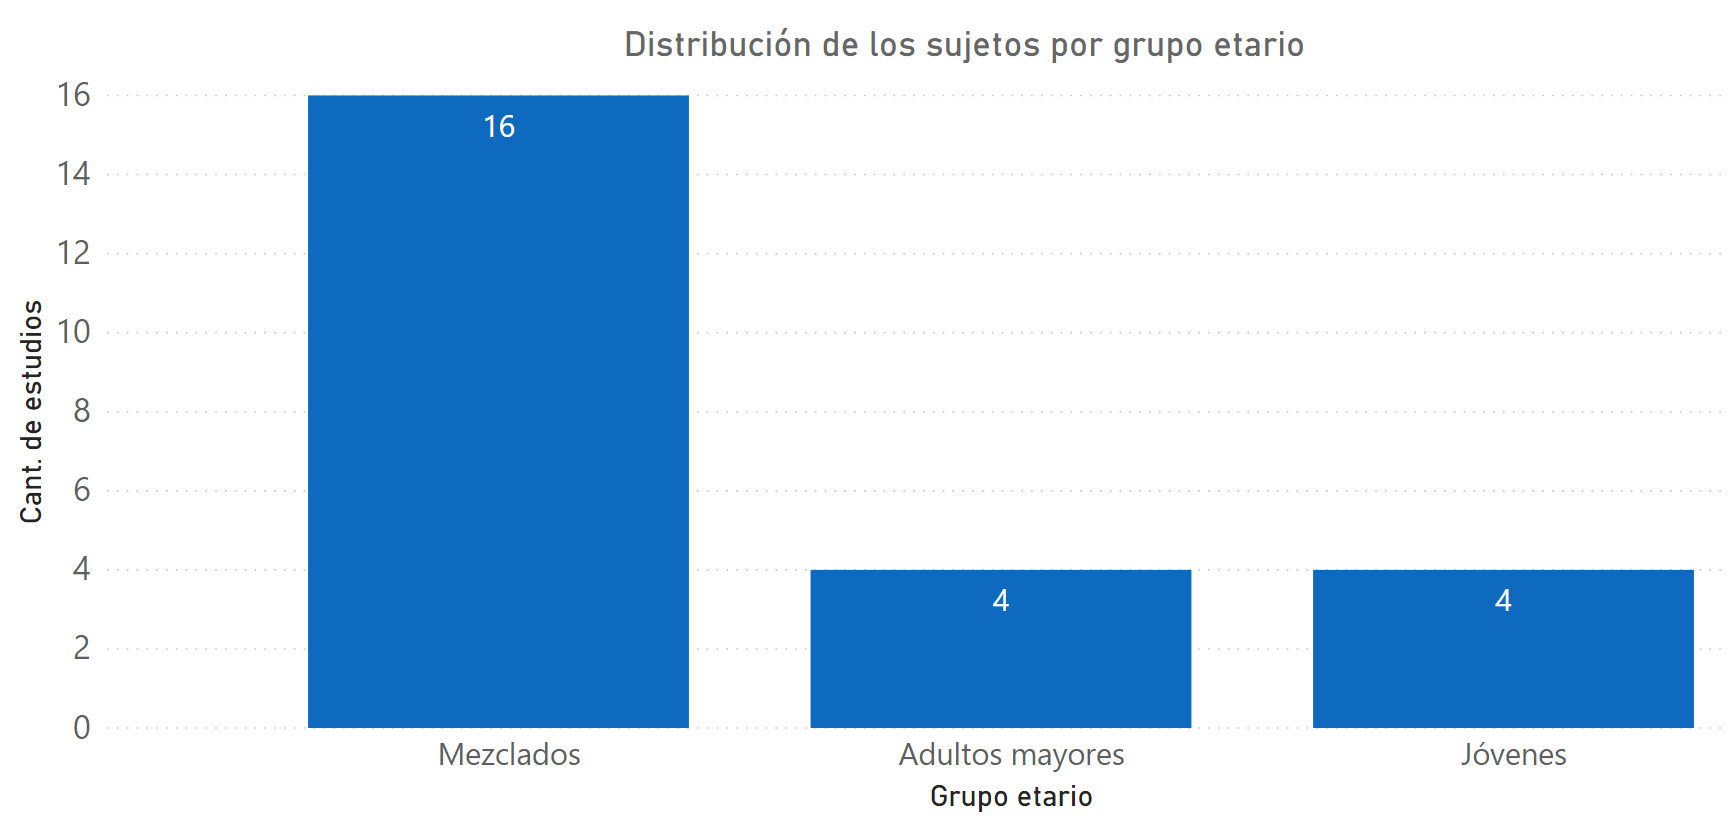
\includegraphics[width=\textwidth]{TESIS/imagenes/chap03/sintesis_grupoEtario.PNG}
\caption{Resumen de la población de estudio por grupo etario.}\label{fig:subjects-age}
\end{figure}

Respecto a la condición de clínica de los sujetos participantes, se puede observar una ligera inclinación a realizar pruebas con personas completamente sanas (41.7\%), aunque existe una proporción muy parecida de los estudios que se realizaron con sujetos enfermos (25\%) o con ambas condiciones (33.3\%) -ver gráfica en Fig. \ref{fig:subjects-condition}-. 

\begin{figure}[H]
\centering
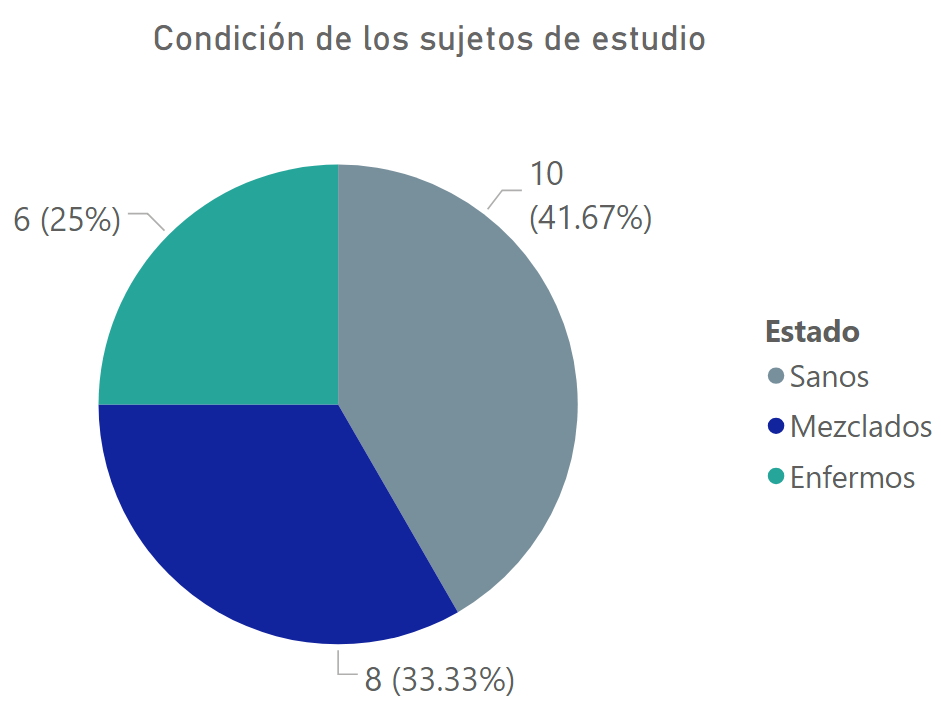
\includegraphics{TESIS/imagenes/chap03/sintesis_subjects.PNG}
\caption{Resumen de condición sobre la totalidad de sujetos en cada estudio}
\label{fig:subjects-condition}
\end{figure}

\noindent Las métricas obtenidas respecto a los sujetos de las pruebas en las distintas investigaciones responden al contexto de investigación, en su totalidad son estudios de ``gait analysis'' con una finalidad médica, aunque no todos para una alteración de la marcha. Por lo tanto, no necesariamente se requieren pruebas con sujetos enfermos.

\section{Limitaciones}\label{synthesis_2}

El presente estudio integra distintos conceptos que requieren un nivel medio a alto de entendimiento, como los son los algoritmos físico-matemáticos necesarios para detectar los eventos del ciclo de la marcha -HS, TO, Stance, Swing-, los métodos numéricos capaces de estimar los parámetros espacio-temporales (i.e. velocidad de la marcha), la biomecánica, y el manejo de múltiples señales de los distintos sensores del IMU. Se reconoce el no cumplimiento de estos requerimientos y un aprendizaje en el transcurso de la SLR. 

En muchos casos no fue posible acceder al estudio completo. Este tipo de situaciones se da cuando la temática tratada tiene un alto impacto comercial y es necesario abonar una suma de dinero a cambio del material completo.

En general, los artículos analizados se enfocan en innovación, presentan una nueva combinación de técnicas para predecir eficazmente alguna de las fases del ciclo de la marcha o al menos un parámetro espacio-temporal. Si bien algunos investigadores proponen nuevos modelos, los esfuerzos se centran principalmente en encontrar y optimizar técnicas de estimación.

\section{Resultados secundarios}

Consecuentemente, se obtuvieron diversos resultados sumamente valiosos, que no fueron planificados al inicio del proyecto mediante preguntas de investigación. De esta manera, se listan los resultados adicionales de la revisión sistemática realizada:
\begin{enumerate}
    \item \underline{Identificación de las compañías de soluciones de sensores.} De gran utilidad para efectuar una amplia comparación de dispositivos existentes en el mercado y poder seleccionar el adecuado.
    \item \underline{Posiciones oportunas del IMU en el pie.} Las estimaciones resultantes de los algoritmos numéricos se ven afectadas por la localización del dispositivo en el cuerpo a sensar. De esta manera, se pudo analizar las distintas localizaciones que lograron mejores resultados y contemplarlas en la solución. 
    \item \underline{Particionamiento del ciclo de la marcha.} Se constato la diversidad de granularidades de las fases de la marcha (i.e. dos,tres, cuatro, cinco, seis, siete y ocho) cada una con sus ventajas y desventajas; la cual permite definir las fases necesarias y suficientes a identificar mediante el sistema PARKIBIP.
    \item \underline{Métodos de estimación de fases de la marcha.} Existen diversos algoritmos innovadores para estimar las fases del ciclo de la marcha, que serán tenidos en cuenta para lograr una solución eficaz.
    \item \underline{Métodos de estimación de parámetros espacio-temporales.} Similar al punto previo, se detectaron variadas técnicas innovadores para estimar los parámetros espacio-temporales de la marcha. En ambas ocasiones, no existe una regla de oro, y todo indica que el campo de estudio es emergente.
    \item \underline{Requerimiento de un algoritmo eficaz de orientación.} Trabajar con el movimiento de un cuerpo particular mediante dispositivos sujetos al mismo, requiere la identificación de la orientación de los dispositivos -por ende la del cuerpo-, respecto a un sistema de referencia inercial (en general, el sistema tierra). Existen diferentes métodos para computar la orientación, basados en rotaciones clásicas hasta sistemas complejos como el gradiente descendente. Es sabido que, en los sistemas de gait analysis, un cuello de botella para estudiar parámetros de la marcha es logra un resultado sumamente eficaz de la orientación del cuerpo respecto al sistema de referencia inercial. Será uno de los desafío de PARKIBIP obtener tal resultado.
    \item \underline{Conocimiento, desafíos y riesgos.} El hecho de analizar detalladamente diversas investigaciones (aproximadamente 85) trae como consecuencia directa la adquisición de conocimiento, por consiguiente las dificultades y riesgos a contemplar y mitigar durante el transcurso del proyecto. Como por ejemplo la implementación de un filtro eficaz y eficiente de Orientación, frecuencias adecuadas por tipo de sensor (acelerómetro, giroscopio, magnetómetro), la necesidad de algoritmos de predicción para parámetros espacio-temporales (es decir, si bien se cumplen las leyes mecánicas, las mismas no son aplicables computacionalmente por el error cuadrático acumulativo). 
\end{enumerate}